% Original editable vector diagram. Compile standalone to regenerate the PDF.
\documentclass[tikz,border=3pt]{standalone}
\usepackage[T1]{fontenc}
\usepackage{lmodern}
\usetikzlibrary{arrows.meta,positioning,calc}
\definecolor{host}{HTML}{967230}
\definecolor{net}{HTML}{007F9A}
\definecolor{sect}{HTML}{71558B}
\definecolor{geom}{HTML}{526579}
\definecolor{event}{HTML}{B94F2F}
\definecolor{atlas}{HTML}{28785D}
\begin{document}
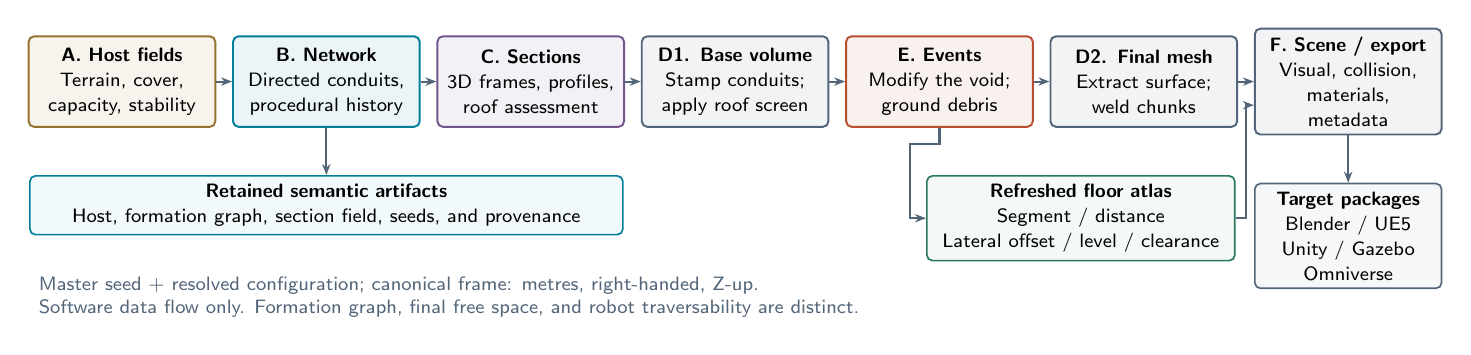
\begin{tikzpicture}[
  font=\sffamily\fontsize{7.5}{9}\selectfont,
  stage/.style={draw=#1,fill=#1!8,rounded corners=2pt,line width=.7pt,
    text width=2.16cm,minimum height=1.15cm,align=center,inner sep=3pt},
  flow/.style={-{Stealth[length=4pt]},line width=.75pt,draw=geom},
  aux/.style={draw=#1,fill=#1!5,rounded corners=2pt,line width=.6pt,align=center,
    minimum height=.67cm,inner sep=3pt}
]
\node[stage=host] (a) at (0,0) {\textbf{A. Host fields}\\Terrain, cover,\\capacity, stability};
\node[stage=net,right=2mm of a] (b) {\textbf{B. Network}\\Directed conduits,\\procedural history};
\node[stage=sect,right=2mm of b] (c) {\textbf{C. Sections}\\3D frames, profiles,\\roof assessment};
\node[stage=geom,right=2mm of c] (d1) {\textbf{D1. Base volume}\\Stamp conduits;\\apply roof screen};
\node[stage=event,right=2mm of d1] (e) {\textbf{E. Events}\\Modify the void;\\ground debris};
\node[stage=geom,right=2mm of e] (d2) {\textbf{D2. Final mesh}\\Extract surface;\\weld chunks};
\node[stage=geom,right=2mm of d2] (f) {\textbf{F. Scene / export}\\Visual, collision,\\materials, metadata};
\foreach \source/\target in {a/b,b/c,c/d1,d1/e,e/d2,d2/f}
  \draw[flow] (\source) -- (\target);
\node[aux=net,text width=7.32cm,below=6mm of b] (sem) {\textbf{Retained semantic artifacts}\\Host, formation graph, section field, seeds, and provenance};
\draw[flow] (b) -- (sem);
\node[aux=atlas,text width=3.7cm,below=6mm of d2,xshift=-8mm] (at) {\textbf{Refreshed floor atlas}\\Segment / distance\\Lateral offset / level / clearance};
\draw[flow] (e.south) -- ++(0,-2mm) -| ([xshift=-2mm]at.west) -- (at.west);
\draw[flow] (at.east) -- ++(1.3mm,0) |- ([yshift=-3mm]f.west);
\node[aux=geom,text width=2.16cm,below=6mm of f] (out) {\textbf{Target packages}\\Blender / UE5\\Unity / Gazebo\\Omniverse};
\draw[flow] (f) -- (out);
\node[anchor=north west,align=left,font=\sffamily\fontsize{7}{8.5}\selectfont,text=geom]
  at ([yshift=-4mm]sem.south west)
  {Master seed + resolved configuration; canonical frame: metres, right-handed, Z-up.\\
  Software data flow only. Formation graph, final free space, and robot traversability are distinct.};
\end{tikzpicture}
\end{document}
